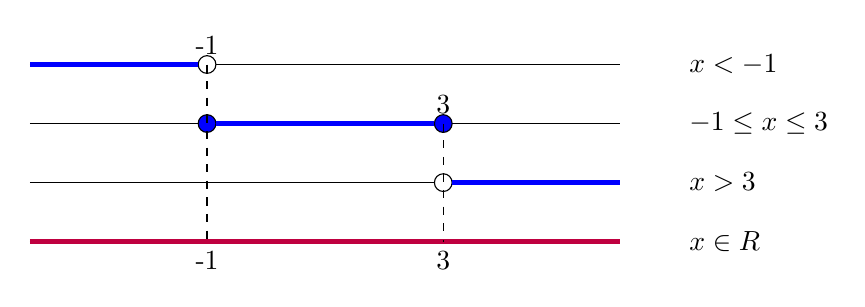
\begin{tikzpicture}[scale=0.75]
            %\draw (-11,0)-- (3,0); %AXIS
            %\foreach \x in {-1} {
            %    \draw (\x,0.5) -- (\x,-0.5) node[below] {$\x$};
            %}
            \draw (-4,1) -- (6,1);
            \draw[fill=white] (-1,1) circle (0.15) node[above]{-1};
            \node[anchor=west, right] at (7,1) {$x < -1$};
            \draw (-4,0) -- (6,0);
            \draw[fill=blue] (-1,0) circle (0.15);
            \draw[fill=blue] (3,0) circle (0.15) node[above]{3};
            \node[anchor=west, right] at (7,0) {$-1 \leq x \leq 3$};
            \draw (-4,-1) -- (6,-1);
            \draw[fill=white] (3,-1) circle (0.15);
            \draw (-4,-2) -- (6,-2);
            \node[anchor=west, right] at (7,-1) {$x > 3$};
            \draw[ultra thick, blue] (-1.15,1) -- (-4,1);
            \draw[ultra thick, blue] (-0.85,0) -- (2.85,0);
            \draw[ultra thick, blue] (3.15,-1) -- (6,-1);
            \draw[ultra thick, purple] (-4,-2) -- (6,-2);
            \node[anchor=west, right] at (7,-2) {$x \in \mathbb{R}$};
            \draw[dashed] (-1,1) -- (-1,-2) node[below]{-1};
            \draw[dashed] (3,0) -- (3,-2) node[below]{3};
\end{tikzpicture}